%=======================================================================
% Declarações iniciais identificando a classe de documento e
% selecionando alguns pacotes adicionais.
%
% As opções disponíveis (separe-as com vírgulas, sem espaço) são:
% - twoside: Formata o documento para impressão frente-e-verso
%   (o default é somente-frente)
% - english,brazilian,french,german,etc.: idiomas usados no documento.
%   Deve ser colocado por último o idioma principal.
%=======================================================================
\documentclass[twoside,english,brazilian]{UNISINOSartigo}
\usepackage[utf8]{inputenc} % charset do texto (utf8, latin1, etc.)
\usepackage[T1]{fontenc} % encoding da fonte (afeta a sep. de sílabas)
\usepackage{graphicx} % comandos para gráficos e inclusão de figuras
\usepackage{bibentry} % para inserir refs. bib. no meio do texto

\usepackage{adjustbox}

\unisinosbst

%================================================================
% Início do documento.
%================================================================
\begin{document}
\titulo{Insight: Um modelo acessível para localização em ambientes internos usando a tecnologia Bluetooth Low Energy}
\autor{Paulo Henrique Grolli Gräbin\footnote{Aluno do curso de Ciência da Computação.  Email: paulograbin@gmail.com}}
\autor{Cristiano André da Costa\footnote{Orientador, professor da Unisinos, doutor em Ciência da Computação pela Universidade Federal do Rio Grande do Sul (2008), Mestre em Ciência da Computação pela mesma Universidade (1997). Email: cac@unisinos.br}}

%=======================================================================
% Resumo em Português.
%=======================================================================
\begin{abstract}
Deficientes visuais passam por grandes dificuldades durante seu deslocamento, devido ao fato de não poderem contar com a sinalização visual, que frequentemente é a única disponível. Aliado a isso, sistemas de posicionamento comumente fazem uso da tecnologia GPS, que se prova insuficiente em ambientes internos. Visando mitigar esse problema, este trabalho tem como objetivo descrever um modelo computacional denominado Insight. O Insight foi desenvolvido para ser utilizado por pessoas com deficiência visual, fornecendo uma localização confiável e um deslocamento seguro através de instruções de voz, leitura de tela e feedback tátil, permitindo que seus usuários possam se deslocar em ambientes desconhecidos sem a necessidade de auxílio de outras pessoas. O modelo é baseado em uma estrutura de serviço na nuvem, contando com servidores distribuídos, onde os clientes são dispositivos móveis que contemplam diversas formas de interação, afim de possibilitar da forma mais natural possível a integração do sistema com a vida diária do usuário. Para a avaliação do modelo foi TODO:... Os resultados obtidos foram TODO:...

\palavraschave{Acessibilidade Ubíqua\@.  Deficiência Visual\@.  Sistemas de Posicionamento Indoor.}
\end{abstract}

%=======================================================================
% Introdução
%=======================================================================
\section{Introdução}
A visão é o recurso mais importante na localização de um indivíduo e na percepção do que se passa ao seu redor. Frequentemente, a sinalização destinada a orientação em locais como aeroportos, shopping centers e universidades é composta inteiramente por sinais visuais. Por esse motivo, pessoas com deficiência visual (PDV) tem grande dificuldade quando necessitam se deslocar, precisando do auxílio de ferramentas como bengalas e cães-guia ou ainda da ajuda de outras pessoas.

\section{Fundamentação Teórica}
Este capítulo apresenta a base teórica sobre a qual está construído este trabalho. Inicialmente são abordados os conceitos de computação ubíqua, computação móvel e acessibilidade. Em seguida esses conceitos são mesclados, sendo introduzido o conceito de acessibilidade ubíqua e tecnologias assistivas. Finalmente, é introduzida a tecnologia Bluetooth, seu modo de funcionamento e aplicações praticas.

\subsection{Computação Móvel e Ubíqua}
Olhando para o futuro, quando existiriam tecnologias tão avançadas, tão conectadas e tão naturalmente integradas em nosssas vidas que nem perceberiamos sua presença, \citetexto{Weiser1991} criou o termo computação ubíqua. 

Weiser antecipou um mundo onde computadores deixariam de possuir apenas o tamanho de um notebook usado em cima de uma mesa. Um mundo onde computadores seriam pequenos o suficiente para serem embutidos em botões de uma camisa e também grandes o suficiente para ocupar os ambientes em que trabalhamos ou estudamos. Tais computadores conversariam entre si de maneira continua e transparente, de modo que seus usuários estariam permanentemente conectados e acessiveis em todos os lugares e em todos os momentos. TODO: Citar a terceira lei de Clarke. Tal definição vai ao encontro do conceito estabelecido por \citetexto{Satyanarayanan2001} para computação móvel como sendo: “Informação na ponta dos dedos, em qualquer lugar e em qualquer tempo”.

Um dos aspectos mais interessantes da computação ubíqua é a ciência de contexto, definida em \citetexto{dey2001understanding} como o uso de informações relevantes, tais como localização, preferência, histórico e horário podem ser usadas para determinar a situação em que o usuário se encontra. Tais informações servem para que os softwares desenvolvidos possam se adaptar as necessidades e reagir, instantânea e transparentemente, às mudanças no ambiente em que o usuário se encontra.

Com a computação cada vez mais onipresente, juntamente com dispositivos móveis e poderosos, é possível aplica-la na tentativa de melhorar a vida das pessoas. Uma das possíveis aplicações é na promoção da acessibilidade de quem necessita. 

\subsection{Acessibilidade}
Acessibilidade representa o direito de acessar informações; eliminação de barreiras arquitetônicas; de disponibilização de comunicação; de acesso físico; de equipamentos e programas adequados; de conteúdo e apresentação da informação em formatos alternativos – não se restringindo somente a internet –, a fim de melhorar a qualidade de vida de pessoas com algum tipo de deficiência. \cite{AcessibilidadeBrasil}. 

% Legislação
No Brasil existe legislação específica para assegurar os direitos individuais de todos os cidadãos. Como exemplo podem ser citadas a lei 5.296/2004, conhecida como lei da acessibilidade, e as leis 10.048/00 e 10.098/00. Juntas, estabelecem normas e critérios básicos para a promoção da acessibilidade, descrevendo regras de construção de espaços públicos, edifícios de uso público e privado. Elas ainda regulamentam como deve se dar a acessibilidade nos sistemas públicos de comunicação e sinalização e normas para promoção da acessibilidade. Também podem ser citados os Decretos 3.298/99 e 5.296/04, que caracterizam o que é deficiência, bem como o que é necessário para que alguém seja considerado pessoa portadora de deficiência física. No aspecto tangível, a legislação brasileira é eficaz ao garantir direitos dos PDV.

% Acessibilidade na tecnologia
Entretanto, a vida digital foge da alçada da jurisdição de qualquer país. Em busca de tornar a internet um lugar mais acessível para todas as pessoas, entram em cena organizações como o Institute of Electrical and Electronics Engineers (IEEE) e o World Wide Web Consortium (W3C), que publicam orientações e diretrizes numa tentativa de garantir acessibilidade universal da web. Nenhuma empresa ou desenvolvedor é formalmente obrigado a aplicar essas diretrizes em seus sites e produtos, todavia, o fazem com o objetivo de atrair mais clientes ou visitantes. As recomendações não são direcionadas para uma tecnologia específica, podendo ser utilizadas em qualquer aplicação, linguagem ou navegador de internet. \cite{W3Cguideliness}. Segundo \citetexto{rodriguez2014accessible}, um aspecto que deve ser considerado é que a aplicação seja acessível para um grande número de pessoas, independentemente das necessidades dos usuários, devendo-se usar diversos canais sensoriais (visual, auditivo e tátil) para passar as informações. Porém, é importante ressaltar que a acessibilidade da web não é baseada apenas na acessibilidade do conteúdo disponibilizado, e sim nos diversos agentes e componentes, como navegadores, usuários, desenvolvedores e ferramentas de desenvolvimento, trabalhando juntos para oferecer uma melhor experiência ao usuário.

De acordo com \citetexto{vanderheiden2008ubiquitous}, no início dos anos 90 apenas computadores fabricados pela Apple contavam com recursos de acessibilidade, enquanto nos demais, softwares de terceiros eram a alternativa para aqueles que necessitavam. Graças aos esforços combinados da indústria e da academia, hoje todos os maiores sistemas operacionais possuem recursos de acessibilidade, como leitores de tela e lente de aumento, nativos entre suas funcionalidades. Pensados e concebidos diretamente na construção do sistema operacional, esses recursos são capazes de oferecer uma integração mais profunda com o sistema e uma experiência muito melhor ao usuário se comparados a softwares produzidos por outras empresas. 

Em consonância com a afirmação de \citetexto{Weiser1991}, \citetexto{vanderheiden2008ubiquitous} diz que, com a computação substituindo o paradigma de computação pessoal para computação ubíqua, é necessário pensar em novas formas de acessibilidade:

\begin{quote}
	Algum dia computadores serão como as lâmpadas de hoje. Houve uma época em que tínhamos que carregar lâmpadas conosco a qualquer lugar que fossemos. As pessoas carregavam consigo lanternas ou velas pelos quartos ou a qualquer lugar onde quisessem ir. Não havia expectativa de que luz seria fornecida a menos que cada um trouxesse a sua. Hoje em dia, ninguém mais carrega lâmpadas. As pessoas esperam que, exceto quando acampando ou viajando pela floresta, diversas fontes de luz sejam oferecidas nos lugares onde elas entram. No futuro podemos esperar uma situação semelhante em relação à computação. Onde quer que se vá, a computação estará através de diversos tipos de interfaces. Talvez tenhamos que levar conosco tipos específicos de interfaces se assim desejarmos, mas seremos capazes de usá-las juntamente com os recursos dos ambientes em que estaremos. \cite{vanderheiden2008ubiquitous}
\end{quote}

Assim emergem os conceitos de acessibilidade ubíqua e interfaces de usuário plugáveis, como talvez a forma definitiva de acessibilidade. Esses conceitos são descritos por \citetexto{Tavares2011} como a capacidade de invocar recursos assistivos especiais diretamente da internet para serem usados em qualquer tela próxima.

\citetexto{Tavares2011} define a acessibilidade ubíqua, também chamada de u-accessibility, como a união entre as normas e padrões para acessibilidade; tecnologias e interfaces que atendem às necessidades dos usuários; e computação ubíqua, através de dispositivos móveis, sensores e a comunicação entre eles.

\subsection{Tecnologias Assistivas}
\citetexto{pupo2006acessibilidade} afirma que existem tecnologias assistivas para auxiliar no acesso às informações, na comunicação, durante a locomoção e em atividades comuns no dia-a-dia, como estudo, trabalho e lazer, citando como exemplos cadeiras de rodas, bengalas, próteses, lupas e aparelhos auditivos. Conforme \citetexto{dias2015navpal}, tecnologias assistivas desempenham um papel chave na independência e segurança de pessoas com deficiência. Para os PDV, tecnologias assistivas bem planejadas e bem implementadas podem fazer significante diferença na educação, aceitação social e produtividade. \cite{dias2015navpal}. Tecnologias assistivas são formas bastante eficazes de promoção de acessibilidade.

Não há um conceito universalmente estabelecido e aceito de tecnologias assistivas. Diversas entidades e países buscam estabelecer sua própria definição. O Brasil apresenta seu conceito em \cite{TA2009}, descrevendo-o como se segue:
\begin{quote}
	Tecnologia Assistiva é uma área do conhecimento, de característica interdisciplinar, que
	engloba produtos, recursos, metodologias, estratégias, práticas e serviços que objetivam promover
	a funcionalidade, relacionada à atividade e participação, de pessoas com deficiência,
	incapacidades ou mobilidade reduzida, visando sua autonomia, independência, qualidade de vida e
	inclusão social
\end{quote}

Conforme \citetexto{stewart2008accessible}, é preferência dos usuários, tanto PDV como aqueles com visão saudável, carregar consigo dispositivos que caibam em um bolso, deixando as mãos livres. O autor ainda afirma que PDV consideram essencial que os aparelhos sejam imperceptíveis durante seu uso. No mesmo sentido, \citetexto{taylor2012smart} diz que PDV preferem não atrair atenção para si enquanto fazem uso de um sistema de localização.

Diversos autores destacam as vantagens do uso de smartphones como dispositivos capazes de oferecer acessibilidade em diversas formas aos usuários. Segundo \citetexto{Ganz2014}, smartphones, item básico possuído por grande parte da população, têm se mostrado uma ferramenta capaz de beneficiar enormemente os PDV em sua vida diária, através de aplicações, como leitores de cédulas de dinheiro, reconhecimento de cores e objetos, navegação na web, leitura de e-mails e ligações telefônicas. O trabalho ainda afirma que o uso de smartphones é possível devido à presença de recursos de acessibilidade oferecidos pelos principais sistemas operacionais disponíveis. Entre esses recursos, podemos destacar a leitura de telas e os alertas vibratórios, essenciais para aqueles que não enxergam as telas sensíveis ao toque que equipam a grande maioria dos smartphones disponíveis atualmente. Ao invés de apenas ler o texto sendo exibido, essa funcionalidade também informa sobre os tipos de cada componente, possibilitando ao usuário saber como interagir com cada um.

De acordo com \citetexto{Brady2013}, os maiores sistemas operacionais para dispositivos móveis disponíveis incluem por padrão a funcionalidade de leitura de tela, de maneira a permitir seu uso por usuários PDV. Aparelhos com tela sensível ao toque eram tidos como inacessíveis a usuários cegos, porém interfaces multitoque bem desenhadas aproveitam melhor o tamanho da tela e são preferidos pelos deficientes visuais.

\citetexto{mau2008blindaid} afirma que a utilização de um dispositivo de uso geral possui uma clara vantagem sobre um aparelho específico que os usuários teriam que carregar e aprender a usar. Os autores ainda definem o telefone celular como “a peça de tecnologia mais valiosa para os cegos”. \cite{mau2008blindaid}. Conforme \citetexto{URNA2007}, a comunidade PDV recebeu muito bem o uso de smartphones, e tem categorizado os aparelhos como um computador ideal para acessibilidade.

Segundo o estudo realizado por \citetexto{quinones2011supporting}, PDV possuem o desejo de carregar consigo a menor quantidade possível de equipamento. É necessário criar tecnologias que não sejam um fardo a ser carregado, mas que ofereçam a quantidade apropriada de informações ao usuário. Uma maneira citada pelo autor é a incorporação de tecnologias de navegação em aparelhos que deficientes visuais carreguem consigo normalmente, assim reduzindo o número de objetos que devem ser cuidados. Smartphones se encaixam perfeitamente nessas necessidades, revelando-se como dispositivo perfeito para ser usado no desenvolvimento de novas tecnologias que visam promover acessibilidade.

Em \citetexto{narasimhan2009smartphone} são sugeridos alguns princípios que devem ser seguidos no desenvolvimento de ferramentas assistivas para PDV:
\begin{itemize}
	\item A ferramenta deve possibilitar a independência nas atividades diárias, não exigindo a assistência e/ou acompanhamento de outras pessoas, com deficiência visual ou não.
	\item Evitar adicionar melhoramentos nas bengalas, visto que aumentar o peso ou novas funcionalidades podem influenciar negativamente no uso diário
	\item Usuários devem ter a opção de usar ou não usar as funcionalidades disponíveis. Seu uso não pode ser forçado para não dificultar seu dia-a-dia.
	\item Manter custos baixos é promover a adoção de produtos pra PDV, já que produtos específicos para esse público tendem a ser mais caros.
\end{itemize}

Baseando-se nestes princípios e na capacidade de auxílio dos smartphones, um exemplo de ferramenta assistiva que vem à tona é o uso de dispositivos móveis para que o usuário deficiente visual obtenha sua localização atual e, a partir dela, descubra locais e recursos acessíveis ao seu redor. Tal ferramenta exige a utilização de alguma tecnologia capaz de distinguir e obter a posição do usuário. Uma das tecnologias capazes de atender a essas necessidades é o Bluetooth.

\subsection{Tecnologia Bluetooth}
Bluetooth é uma tecnologia de comunicação sem fios de curto alcance, lançada comercialmente em 1990, quando teve sua primeira especificação formal divulgada. Desde então, diversas modificações foram feitas e a tecnologia passou por diversos aprimoramentos, estando atualmente na versão 4, também conhecida como Bluetooth Smart ou Bluetooth Low Energy, lançada em 2010. A tecnologia nativamente possui capacidade para lidar com diversos serviços, tais como criptografia, transferência de arquivos e transferência síncrona e assíncrona de dados.

O Bluetooth foi criado e atualmente é mantido por um conjunto de empresas conhecido como Bluetooth Special Interest Group (SIG). Inicialmente formado por Ericsson, Intel, Nokia, Toshiba e IBM, o SIG é hoje composto por mais de 20.000 empresas, incluindo Apple, Microsoft, Motorola e Lenovo.

A tecnologia possui duas formas distintas de atuação, apesar de compartilharem entre si alguns pontos em comum. O primeiro e mais antigo modo, disponível desde a primeira especificação, é chamado Basic Rate (BR). O segundo foi introduzido somente na versão 4 e é chamado Low Energy (LE) e é o modo que será utilizado pelo modelo proposto neste trabalho.

De acordo com \citetexto{Townsend2014}, o LE foi criado para permitir produtos que requerem baixíssimo consumo de energia e baixo custo, quando comparados ao outro modo. Assim sendo, esse modo foi pensado para aplicações que exigem pouca troca de informações. Um exemplo de produto viável com a chegada do modo LE são os beacons Bluetooth, que consistem em dispositivos do tamanho de uma moeda comum, compostos por um processador, uma bateria e um transmissor, que transmitem informações sobre si em intervalos regulares. Como o sinal dos beacons tem seu alcance limitado a alguns poucos metros, foi introduzido o conceito de microlocalização, tornando possível o desenvolvimento de novas aplicações e serviços onde antes não era possível, tais como lojas, grandes shows ou eventos, estádios esportivos e em ambientes internos. A microlocalização é definida por \citetexto{zafari2015micro} como a obtenção da localização de uma entidade com grau de precisão na ordem dos centímetros. 

A imensa maioria dos telefones celulares hoje faz uso nativo da tecnologia, não exigindo qualquer tipo de equipamento adicional. Os sistemas operacionais Android e iOS oferecem suporte a tecnologia a partir das versões 4.3 e 5, respectivamente. Ao contrário da versão anterior, a partir da versão 4, a tecnologia Bluetooth não exige o pareamento de dispositivos para que eles possam se localizar e comunicar.

De acordo com \citetexto{ballance2008developing}, a combinação computação ubíqua e Bluetooth tem potencial para fomentar soluções simples e baratas que outrora não seriam possíveis.

\citetexto{taylor2012smart} revelam que diversas tecnologias foram utilizadas anteriormente em modelos de sistema para localização e navegação para PDV, tanto em ambientes internos como externos. Sonares, Radio Frequency Identification (RFID), Near Field Communication (NFC), Bluetooth e Global Positioning System (GPS) são algumas delas. Os autores ainda apontam que, apesar de todas elas oferecerem vantagens em suas propostas, todas também possuem pontos fracos:

\begin{itemize}
  \item GPS é normalmente usado para localização em ambientes externos, mas se mostra ineficiente devido à própria natureza das ondas de rádio usadas na tecnologia, quando obstáculos são locados ao redor do usuário. De acordo com \citetexto{montague2010accessible}, apesar de GPS ser muito eficiente na hora de determinar um ponto em um mapa, essa tecnologia está longe ser a melhor escolha para ambientes internos. Nesse cenário é preciso viabilizar a possibilidade de diversos andares em um local, o que não é possível ser feito via GPS.
  \item Sonares são formas baratas de detecção de objetos e obstáculos, através de frequências acústicas, mas exigem hardware dedicado e não servem para localização.
  \item RFID, juntamente com NFC, exige proximidade de seus emissores para que a comunicação seja estabelecida.
  \item Os autores não chegam a citar nominalmente os pontos fracos da tecnologia Bluetooth, mas um grande ponto que pode ser citado é o consumo de bateria causado pelas versões que antecederam a versão 4, também chamada de Bluetooth Low Energy.
\end{itemize}

A Tabela \ref{tab:tecnologiasLocalizacao} mostra algumas características dessas tecnologias.

\begin{table}
	\caption{Tabela comparativa entre tecnologias aplicadas em localização}
	\label{tab:tecnologiasLocalizacao}
		\begin{tabular}{ p{2,5cm} | p{2cm} | p{2,5cm} | p{3cm} | p{3cm} }
			\hline
				Tecnologia & Precisão & Abrangência & Suportada por smartphones & Exige linha de visão   \\ \hline
				GPS & 10 m & Externo & Praticamente todos & Não   \\ \hline
				Bluetooth 2 & 100 m & Ambos & Praticamente todos & Não   \\ \hline
				Bluetooth BE & 100 m & Ambos & Alguns & Não   \\ \hline
				RFID & Entre 10cm e 100m & Ambos & Alguns & Não   \\ \hline
				NFC & Até 10 cm & Ambos & Alguns & Não   \\ \hline
				Ultrassom & Centímetros & Ambos & Poucos & Não   \\ \hline
				Infravermelho & Centímetros & Ambos & Poucos & Sim   \\ \hline
			\end{tabular}
		\fonte{\citetexto{stewart2008accessible}}
\end{table}

Analisando a tabela podemos ver que a tecnologia GPS é a que oferece a maior precisão na localização, além de ser suportada pela maioria dos smartphones. Porém, ela não é recomendada para ambientes internos. As tecnologias ultrassom e infravermelho oferecem boa precisão, mas são pouquíssimos os modelos de smartphone que fazem uso delas. Infravermelho ainda exige contato visual direto e sem restrições entre os dispositivos para funcionar. RFID e NFC oferecem ótima precisão devido à proximidade necessária para uso da tecnologia, porém, possuem pouco suporte por parte dos dispositivos. Bluetooth, em ambas as versões, possuem precisão média e são bem suportadas pelos smartphones.

Importante ressaltar que os dados apresentados são limites teóricos da tecnologia obtidos através da especificação de cada uma das tecnologias. Estes valores podem variar para mais ou para menos, visto que, segundo \citetexto{Townsend2014}, o alcance de qualquer tecnologia sem fio é influenciado por diversos fatores, entre eles é possível  citar o ambiente onde ela está sendo utilizada, design da antena e o material utilizado.

\section{Trabalhos Relacionados}
Nesta seção serão apresentados quatro trabalhos relacionados com a solução a ser proposta. A busca por trabalhos foi feita com base na pesquisa pelas palavras-chave TODO: em bases de dadas da área de ciência da computação como ACM\footnote{Disponível em http://dl.acm.org.}, IEEE\footnote{Disponível em http://www.ieee.org.} e no buscador Google Acadêmico\footnote{Disponível em http://scholar.google.com.}. A seleção dos trabalhos foi feita considerando critérios como a similaridade do objetivo com o deste trabalho, o ano de publicação do modelo, suporte à acessibilidade, foco em dispositivos móveis e abrangência em ambientes internos.

Os trabalhos relacionados escolhidos foram: Percept (\cite{Ganz2011} e \cite{Ganz2012}), um modelo de navegação em ambientes internos usando RFID; 
UCAT (\citetexto{ucat2014}), uma aplicação para dispositivos móveis que permite ao usuário saber quem está ao seu redor; 
Development of a Navigation System Using Smartphone and Bluetooth Technologies to Help the Visually Impaired Navigate Work Zones Safely (\citetexto{chen2014}), um modelo para dispositivos móveis que avisa aos usuários sobre sua aproximação de zonas em obras e Tirésias (\citetexto{Falk2013}), um modelo de acessibilidade para dispositivos móveis para o suporte de pessoas que possuem deficiência visual.

Percept é um modelo de localização que busca aumentar a percepção dos PDV. \citetexto{Ganz2011} e \citetexto{Ganz2012} definem um sistema de localização em ambientes internos utilizado através de dispositivos móveis que permite ao usuário selecionar um dos destinos possíveis no ambiente e obter rota e instruções para chegar até ele. O Percept é composto por tags RFID passivas espalhadas pelo ambiente, responsáveis por representar individualmente cada possível destino no ambiente e por indicar ao modelo o destino escolhido pelo usuário; uma luva com hardware customizado, capaz de fazer a leitura das tags e enviar comandos ao dispositivo móvel; um dispositivo móvel, que recebe informações da luva e se comunica com o servidor para obter a rota até o destino escolhido; e o servidor PERCEPT, responsável por armazenar o layout dos ambientes e calcular a rota até o destino escolhido.

UCAT (acrônimo para Ubiquitous Context Awareness Tools for the Blind), proposto por \citetexto{ucat2014}, é um sistema que objetiva diminuir o desconforto dos deficientes visuais permitindo que eles saibam quem está ao seu redor. O modelo usa Bluetooth e o endereço único de cada dispositivo para identificar unicamente cada telefone, que por usa vez é relacionado a um contato na agenda do usuário. A aplicação mostra todos os dispositivos ao redor do usuário, sendo capaz de detectar quando alguém se aproxima ou se afasta, e permite ao a criação de notas que serão exibidas uma vez que o contato esteja proximo ao usuário. Para facilitar a interação, o modelo lança mão se alguns recursos de usabilidade, tais como navegação por gestos, retorno através de voz e alertas vibratórios.

A proposta de \citetexto{chen2014} propõe um modelo de software para dispositivos móveis que detecta, através de beacons Bluetooth, quando o usuário está se aproximado de zonas em obras, de maneira a alertar verbalmente o usuário sobre o possível perigo a frente. O modelo consiste em três componentes: servidor, possuindo com o banco de dados dos mapas e zonas em obras; aplicativo para Android que constantemente busca pro sinais Bluetooth nas proximidades do usuário e se comunica com o banco de dados e os beacons; e os beacons propriamente ditos, espalhados nos limites das zonas em obras e escolhidos devido a possíveis problemas com o sinal de GPS. A inclusão e manutenção das zonas é feita através de uma aplicação web armazenada no servidor e acessada através de um computador comum qualquer.

A proposta de \citetexto{Falk2013}, denominada Tirésias, é baseado no modelo Hefestos, proposto por \citetexto{Tavares2011}. Este, por sua vez, é um modelo genérico que visa estabelecer padrões de acessibilidade que possam ser aplicados em diversos tipos de deficiência. Segundo os autores, o Tirésias pode ser compreendido como uma especialização do Hefestos para atender as necessidades das pessoas com deficiência visual. O modelo obtém a posição atual do usuário através do GPS contido no smartphone e, se baseando nela, exibe recursos de acessibilidade disponíveis nas proximidades. Algumas das funcionalidades oferecidas são a listagem de recursos disponíveis, a indicação de caminho até o recurso selecionado e a solicitação de ajuda. O modelo é composto pelos módulos de saída, responsável por gerenciar as informações passadas ao usuário; entrada, responsável por gerenciar a interface com o usuário; configurações, que disponibiliza ajustes de forma a customizar o sistema às necessidades do usuário; pelo assistente pessoal, responsável pela comunicação com o Hefestos, através da qual são obtidos perfis de usuário e recursos disponíveis para o suporte à acessibilidade; somados ao modelo Hefestos. De acordo com \citetexto{Falk2013}, o Tirésias emprega sensibilidade ao contexto e acessibilidade ubíqua, utilizando maneiras especializadas de interação com o sistema, para promover acessibilidade aos PDV.





Prevendo uma maior facilidade e compreensão quanto à comparação entre os trabalhos relacionados, foi elaborada a TODO:. Nela são destacadas as principais características e aspectos considerados relevantes para o presente trabalho.

\begin{table}
	\caption{Tabela comparativa entre os trabalhos relacionados}
	\label{tab:trabalalhosRelacionados}
	\centering%
	\begin{minipage}{1\textwidth}
		\begin{adjustbox}{max width=\textwidth}
		\begin{tabular}{ p{3cm} | p{3cm} | p{3cm} | p{3cm} | p{3cm} }
 	\hline
 	& Percept & UCAT & Navigation System for Workzone & Tirésias \\ \hline
	Método de localização & RFID & Bluetooth 2.1 & Bluetooth LE & GPS \\ \hline
	Abrangência & Indoor & Indoor e outdoor & Zonas em obras & Indoor \\ \hline
	Ambientes dinâmicos & Não especificado & Não especificado & Não especificado & Não especificado \\ \hline
	Meio de acesso & Dispositivos móveis & Dispositivos móveis & Dispositivos móveis & Dispositivos móveis \\ \hline
	Interface do utilizador & Toques & Toques e gestos & Toques & Toques e gestos \\ \hline
	Hardware específico & Sim & Não & Não & Não \\ \hline
	Comunicação & Internet ou intranet & Internet & Internet & Internet ou intranet \\ \hline
	Interoperabilidade & Não & Não & Não & Sim, através de agentes \\ \hline
	Adaptação & Não & Sim, através de sensibilidade ao contexto & Não & Sim, através de sensibilidade ao contexto \\ \hline
	Banco de dados & Postgres & SQLite & MySQL & Não especificado \\ \hline
	Linguagem & Java & Java & Java & Objective-C \\ \hline
	Sistema operacional & Android & Android & Android & iOS \\ \hline
	Bibliotecas utilizadas & Não especificado & Não especificado & Não especificado & Não especificado \\ \hline
	Hardware & Luva equipada c/ leitor RFID e dispositivo móvel c/ Bluetooth & Dispositivos móveis c/ Bluetooth & Dispositivos móveis c/ Bluetooth & Dispositivos Móveis c/ GPS \\ \hline
	Arquitetura & Cliente-servidor & Cliente-servidor & Cliente-servidor & Cliente-servidor \\ \hline
		\end{tabular}
		\end{adjustbox}
		\fonte{Elaborado pelo autor.}
	\end{minipage}
\end{table}



Baseado nas lacunas observadas, o presente trabalhos busca integrar, em uma única solução para dispositivos móveis, ...



\section{Modelo Proposto}

\section{Avaliação}

%=======================================================================
% Conclusão
%=======================================================================
\section{Conclusão}




% \section{Introdução}

% \begin{itemize}
% 	\item Cada transicão de tela tem uma fala

%     //TODO: todo android vem com o sintetizador de voz
%     //TODO: inspiração veio quando minha namorada comentou que viu no trem...

%     //TODO: navigation, initicializa já no primeiro lugar do camihno
%     //TODO: app roda no plano de fundo

%         // TODO: No primeiro uso, pergunta se o usuário quer que o aplicativo monitore sua região e
%     // se auto execute quando chega na área
% \end{itemize}

% Conforme , a introdução tem o objetivo de ``\emph{introduzir} o material que vai ser apresentado em mais detalhe nas seções subseqüentes''. Na introdução você deve contextualizar o problema e mostrar por que vale a pena resolvê-lo. Você deve apresentar a solução proposta e mostrar o seu diferencial em relação aos trabalhos relacionados. Observe, porém, que na introdução você deve apenas tratar do O QUÊ e PORQUÊ, sem tratar do como, que deve ser explicado na seção que descreve o trabalho desenvolvido.

% Geralmente, a introdução tem uma estrutura similar ao resumo e deve apresentar:
% \begin{itemize}
% 	\item \textbf{Contexto e motivação:} Aqui você deve apresentar o contexto do trabalho (área de que ele se trata) e uma motivação para trabalhar nesse assunto.
% 	\item \textbf{Problema:} Aqui você vai apresentar um problema, uma lacuna, observada na área e que você pretende tratar. Você deve se perguntar aqui: ``Que respostas estou disposto a responder?''. O problema deve ser definido claramente e delimitado em termos de espaço de tempo. Veja que essa parte visa alertar o leitor de que o que você está propondo é uma solução para um problema observado na área. 
% 	\item \textbf{Objetivos:} Aqui você deve apresentar os objetivos do seu trabalho. Tome cuidado para não confundir objetivos com atividades.   Faça a si mesmo a pergunta: ``O que pretendo alcançar com a pesquisa?''. Você pode discernir entre objetivos gerais e objetivos específicos:
% 	\begin{itemize}
% 		\item Objetivo geral --- qual o propósito da pesquisa?
% 		\item Objetivos específicos --- abertura do objetivo geral em outros menores (possíveis capítulos).
% 	\end{itemize}
% 	Veja abaixo um exemplo de objetivo retirado da monografia de {Teixeira09}:

% 	Com a possibilidade de acesso a base de dados XML gerada a partir do Sistema de Currículos Lattes e a necessidade de melhor reutilizar as informações existentes neste sistema, o presente trabalho tem como objetivo geral permitir o acesso do pesquisador a seus dados através de uma interface mais amigável: o padrão LaTeX. Para isto destacam-se os seguintes objetivos específicos:
% 	\begin{alineas}
% 		\item identificar e analisar o formato de especificação de currículos da Plataforma Lattes;
% 		\item disponibilizar uma ferramenta para a geração de uma representação de dados intermediária a partir do formato especificado;
% 		\item implementar a tradução dos dados colhidos em código LaTeX através da utilização da ferramenta criada;
% 		\item analisar os resultados obtidos e as alternativas presentes no uso da ferramenta.
% 	\end{alineas}
% \end{itemize}

% %=======================================================================
% % Escrevendo o Texto
% %=======================================================================
% \section{Escrevendo o Texto}
% Este capítulo apresenta algumas orientações para a escrita do texto.

% \subsection{Comandos do \LaTeX}
% Como regra geral, use os comandos tradicionais do \LaTeX\ para formatar seu texto.  Neste documento procuramos demonstrar os comandos mais comumente utilizados em monografias acadêmicas.

% Neste capítulo apresentamos alguns exemplos de como colocar figuras e tabelas no seu texto.

% \subsection{Ilustrações}
% Aqui são apresentados alguns detalhes sobre o uso de ilustrações.

% \subsubsection{Legendas}
% As legendas das figuras devem se encontrar no topo da figura e não abaixo, como usualmente colocado. Abaixo da figura, é obrigatório colocar a fonte (mesmo que a figura tenha sido do próprio autor).

% As legendas devem conter o tipo da ilustração (Figura, Tabela, etc), seguido de numeração simples (sem número do capítulo).

% Toda figura deve ser citada no texto, como nos exemplos que seguem.

% \subsubsection{Figuras}
% A Figura~\ref{fig:escrita} ilustra as fases psicológicas da escrita da dissertação. Você vai se reconhecer no personagem. ;-)

% % \begin{figure}
% % 	\caption{Fases psicológicas da escrita da dissertação}
% % 	\label{fig:escrita}
% % 	\centering%
% % 	\begin{minipage}{.8\textwidth}
% % 		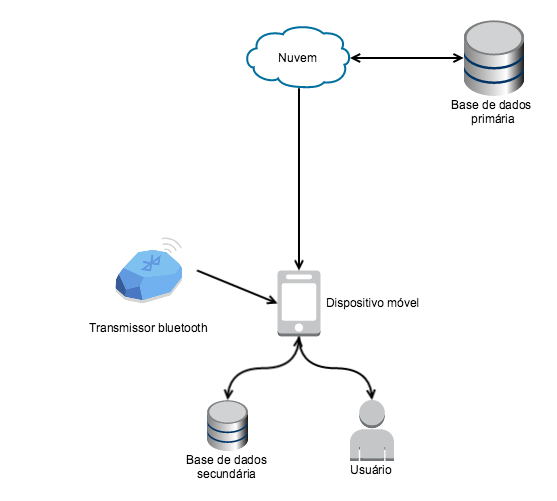
\includegraphics[width=\textwidth]{escrita}
% % 		\fonte Cham12}}
% % 	\end{minipage}
% % \end{figure}

% \subsubsection{Tabelas}
% A Tabela~\ref{tab:estacoes} é um exemplo de tabela elaborada pelo(a) próprio(a) autor(a).

% \begin{table}
% 	\caption{Período das estações do ano no Brasil}
% 	\label{tab:estacoes}
% 	\centering%
% 	\begin{minipage}{.6\textwidth}
% 		\begin{tabular*}{\textwidth}{ll}
% 			\hline
% 			\textbf{Meses} & \textbf{Estações do Ano}\\
% 			\hline
% 			21 de março a 21 de junho & Outono\\
% 			21 de junho a 23 de setembro & Inverno\\
% 			23 de setembro a 21 de dezembro & Primavera\\
% 			21 de dezembro a 21 de março & Verão\\
% 			\hline
% 		\end{tabular*}
% 		\fonte{Elaborada pela autora.}
% 	\end{minipage}
% \end{table}

% \subsection{Resumo}
% % O resumo deve conter de 150 a 250 palavras. No resumo não deve haver citações e indica-se que essa seja a última seção do texto a ser escrita. Veja abaixo uma sugestão de organização e exemplo de resumo de {Moro11}.

% Sugestão (uma a três linhas para cada item):
% \begin{itemize}
% 	\item Contexto geral e específico;
% 	\item Questão/problema sendo investigado (propósito do trabalho);
% 	\item Estado-da-arte (por que precisa de uma solução nova/melhor);
% 	\item Solução (nome da proposta, metodologia básica sem detalhes, quais características respondem as questões iniciais, interpretação dos resultados, conclusões).
% \end{itemize}

% % Exemplo (SANTOS et al., 2008 apud Moro11}):
% \begin{quote}
% CONTEXTO: A Web é abundante em páginas que armazenam  dados de forma implícita. PROBLEMA: Em muitos casos, estes dados estão presentes em textos semiestruturados sem a presença de delimitadores explícitos e organizados em uma estrutura também implícita. SOLUÇÃO: Este artigo apresenta uma nova abordagem para extração em textos semi-estruturados baseada em Modelos de Markov Ocultos (Hidden Markov Models - HMM). ESTADO-DA-ARTE e MÉTODO PROPOSTO: Ao contrário de outros trabalhos baseados em HMM, a abordagem proposta dá ênfase à extração de metadados, além dos dados propriamente ditos. Esta abordagem consiste no uso de uma estrutura aninhada de HMMs, onde um HMM principal identifica os atributos no texto e HMMs internos, um para cada atributo, identificam os dados e metadados. Os HMMs são gerados a partir de um treinamento com uma fração de amostras da base a ser extraída. RESULTADOS: Os experimentos realizados com anúncios de classificados retirados da Web mostram que o processo de extração alcança qualidade acima de 0,97 com a medida F, mesmo se esta fração de treinamento é pequena. 
% \end{quote}

% %=======================================================================
% % Exemplos de Citações e Referências Bibliográficas
% %=======================================================================
% \section{Exemplos de Citações e Referências Bibliográficas}
% \nobibliography* % para usar o \bibentry
% Neste capítulo são apresentados exemplos de citações e referências bibliográficas.  Aqui é utilizado o pacote \texttt{bibentry}, que permite a inserção de referências no meio do texto (atenção para a diferença entre citações e referências).

% Você vai ver que, neste exemplo, não está sendo usado o estilo de referências bibliográficas do projeto ABNTeX\footnote{http://http://sourceforge.net/projects/abntex}.  Você é completamente livre para usá-lo (veja no início do arquivo .tex como fazer isso).  Os motivos para não usar o ABNTeX neste exemplo são basicamente dois:
% \begin{itemize}
% 	\item Para usar o ABNTeX, é necessário instalá-lo em seu sistema \TeX\ primeiro; embora não seja uma tarefa tão complicada, enxergamos como uma dificuldade a mais para o usuário iniciante.  Nosso objetivo aqui é facilitar ao aluno da UNISINOS o uso deste modelo, de modo que basta copiar os arquivos \texttt{UNISINOSmonografia.cls} e \texttt{unisinos.bst} para a pasta onde estão seus arquivos .tex;
% 	\item As normas da ABNT são tão complexas que, para atender a todas as variações possíveis de citações e referências, o projeto ABNTeX criou uma série de campos adicionais nas entradas do arquivo .bib.  Embora funcione para o caso ABNT, o efeito colateral de fazer isso é que o seu arquivo .bib será muitas vezes incompatível com os demais estilos tradicionais do BibTeX, como \texttt{plain}, \texttt{alpha}, \texttt{ieeetr}, entre outros.  Por exemplo, em referências a artigos publicados em conferências, o campo \texttt{organization} é usado pelo ABNTeX para definir o nome do evento.  Isso não é padrão e não será reconhecido pelos estilos tradicionais\footnote{Veja como criar seus arquivos .bib no manual do BibTeX, que pode ser encontrado em http://ctan.tug.org/tex-archive/biblio/bibtex/contrib/doc/btxdoc.pdf.}.  Considerando que um dos maiores benefícios do BibTeX é criar um arquivo .bib que pode ser reutilizado pelo resto da vida, nossa estratégia com o \texttt{unisinos.bst} foi tentar aproximar ao máximo a formatação exigida pela ABNT sem implicar na criação de arquivos .bib incompatíveis.  Isso funciona bem na grande maioria dos casos, mas não em todos.  Nesse caso, a saída é usar o ABNTeX ou então alterar manualmente o arquivo .bbl que é gerado ao rodar o comando \texttt{bibtex}.
% \end{itemize}


% \subsection{Citações}
% As citações podem ocorrer de duas formas: com os nomes dos autores inseridos no texto ou não.  Isso implica em uma construção diferente para as frases.  Por exemplo:

% \subsection{Livros}
% Seguem alguns exemplos de referências de livros:

% \subsection{Artigos em Periódicos}
% Os exemplos abaixo ilustram referências a artigos em periódicos.

% \subsection{Artigos em Conferências}

% \subsection{Teses e Dissertações}
% Seguem algumas referências a trabalhos acadêmicos, como teses, dissertações, trabalhos de conclusão de curso, etc.




%=======================================================================
% Resumo em língua estrangeira (sim, é aqui mesmo).
%
% O idioma usado aqui deve necessariamente aparecer nos parâmetros do
% \documentclass, no início do documento.
%=======================================================================
\begin{otherlanguage}{english}
\titulo{Insight: An accessible model for navigation inside indoor environments using Bluetooth Low Energy}
\begin{abstract}
Este documento apresenta orientações para uso da classe \LaTeX\ de formatação de artigos para a UNISINOS\@.  Ao mesmo tempo, ele serve como exemplo de uso da classe, demonstrando os principais comandos a serem utilizados, e outras orientações mais gerais de uso do \LaTeX.  Adicionalmente, procuramos incluir no documento algumas orientações sobre a escrita da monografia em si, reunindo dicas e recomendações que contribuem para aumentar a qualidade técnica dos trabalhos acadêmicos.  O Resumo deve conter de 150 a 250~palavras e apresentar o objetivo, o método, os resultados e as conclusões do artigo. Deve ser composto por frases concisas e afirmativas. Recomenda-se o uso de parágrafo único. Deve-se usar o verbo na voz ativa e na terceira pessoa do singular.

\palavraschave{Ubiquitous Accessibility\@.  Visual Impairment\@.  Indoor positioning systems  \LaTeX.}

\end{abstract}
\end{otherlanguage}

%=======================================================================
% Referências
%=======================================================================
\bibliography{bibliografia_artigo}

\end{document}